\section{Filtro LDR}
\subsection{Enunciado}

\subsection*{Filtro \textit{LDR}}
  Programar el filtro \textit{LDR} en lenguaje C y en
  ASM haciendo uso de las instrucciones \textbf{SSE}.

\vspace*{0.3cm} \noindent
\textbf{Experimento 1}

  Analizar cuales son las diferencias de performace entre las versiones de C y ASM. 
  Realizar gráficos que representen estas diferencias.
  
\subsection{An\'alisis previo}

\subsection{Implementaci\'on en C}
\paragraph{\textbf{Titulo del parrafo} } Bla bla bla bla.
Esto se muestra en la figura~\ref{nombreparareferenciar}.
\subsection{Implementaci\'on en assembler}
\begin{codesnippet}
\begin{verbatim}

struct Pepe {

    ...

};
\end{verbatim}
\end{codesnippet}
\subsection{Resultado de los experimentos}

\vspace*{0.3cm} \noindent
\textbf{Experimento 1}

\begin{figure}
  \begin{center}
	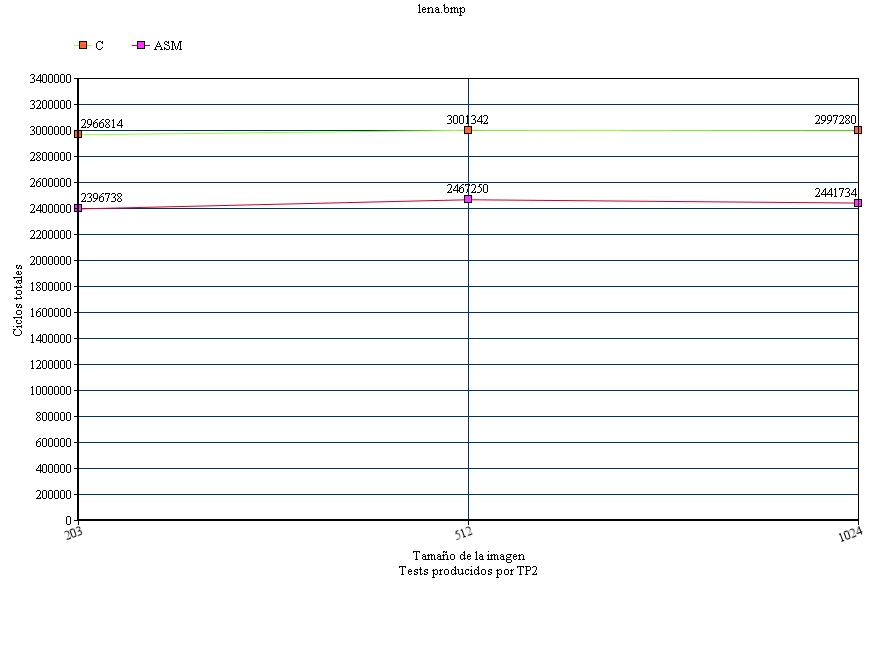
\includegraphics[scale=0.66]{imagenes/ldr-lena.jpg}
	\caption{Lena}
	\label{Lena}
  \end{center}
\end{figure}

\begin{figure}
  \begin{center}
	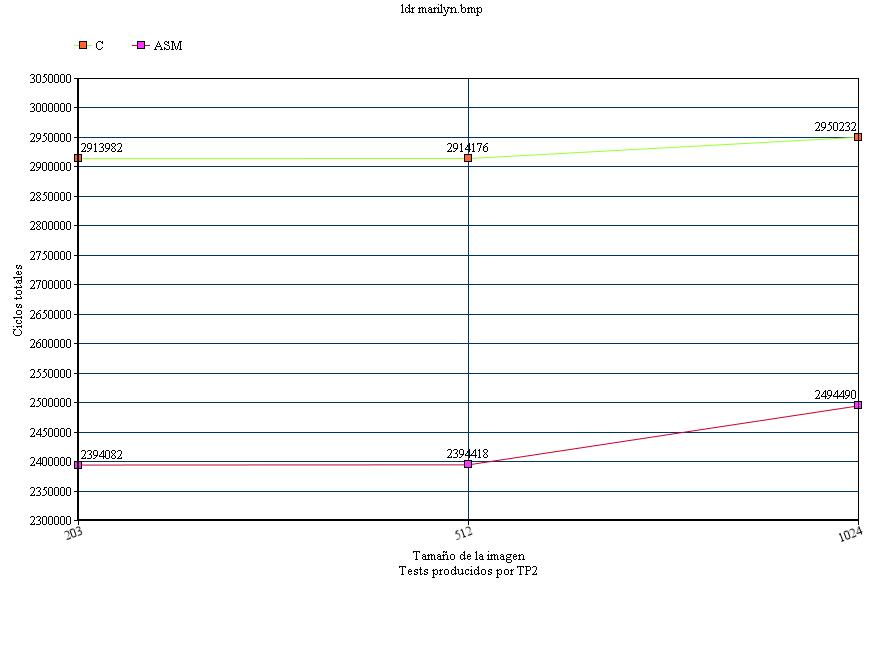
\includegraphics[scale=0.66]{imagenes/ldr-marilyn.jpg}
	\caption{Marilyn}
	\label{Marilyn}
  \end{center}
\end{figure}

Realizamos los tests armando un ciclo de 100000 ejecuciones del mismo c\'odigo con las mismas entradas, y a su vez ejecutamos estos tests 5 veces para cada entrada. \'Esto nos 
permiti\'o hacer promedios y descartar tests que daban muy lejos del valor medio.

Como muestran los gr\'aficos presentados, hay claras diferencias de velocidad (medida en cantidad de ciclos) entre uno y otro lenguaje. Tambi\'en notamos que no hay una gran 
variaci\'on de velocidad entre los distintos tamaños de las im\'agenes, as\'i como a veces las variaciones no son las esperadas. En este sentido, realizamos varias ejecuciones 
del TP2 con exactamente los mismos par\'ametros y vimos que variaban sin un patr\'on. Pensamos que si mejoraba con las sucesivas iteraciones podr\'ia ser 
producto de la acci\'on de la cache, pero como no fue as\'i vemos que tiene que ver con qu\'e tan ocupado est\'a el cpu. \'Esto no pudo ser confirmado ya que todos 
los tests se corrieron sin ningun otro programa visible a nosotros est\'e corriendo..
\begin{figure}
  \begin{center}
	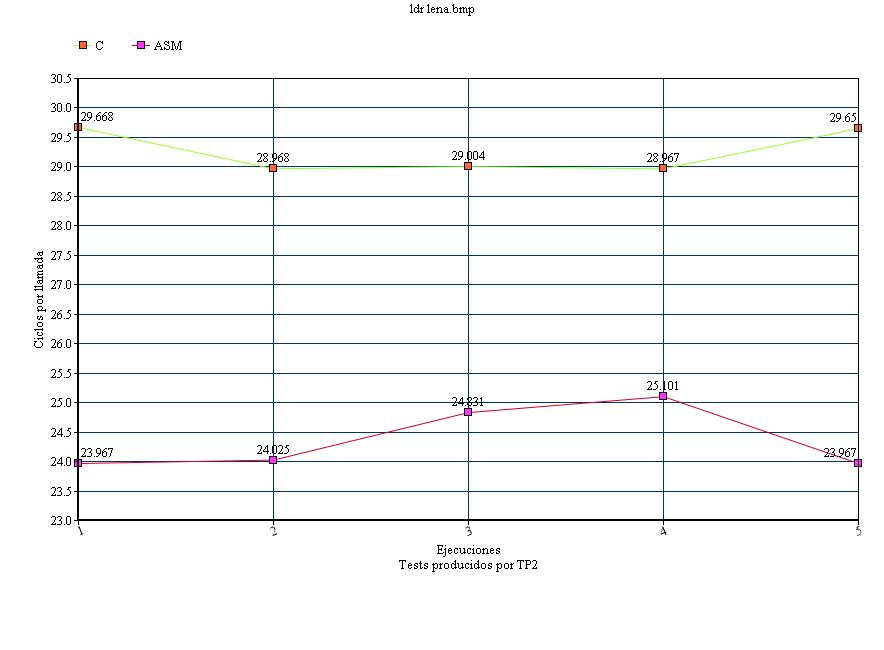
\includegraphics[scale=0.66]{imagenes/ldr-lena-203.jpg}
	\caption{lena-203x203}
	\label{lena-203x203}
  \end{center}
\end{figure}
